\begin{figure}
  \hspace*{30mm}
  \begin{tikzpicture}
    \node[inner sep=0pt] (circuit) at (0,0) {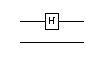
\includegraphics[scale=2, trim={0 0 5mm 0},clip]{Figures/circuits/H_I}};
    \pic (e1) {ebit=e1/5.63mm/13mm};
    \node[right=2mm of circuit.north west, font=\itshape] (text) {a)};
  \end{tikzpicture} 
  \hspace*{10mm}
  \begin{tikzpicture}
    \node[inner sep=0pt] (circuit) at (0,0) {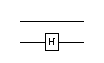
\includegraphics[scale=2, trim={0 0 5mm 0},clip]{Figures/circuits/I_H}};
    \pic (e1) {ebit=e1/5.63mm/13mm};
    \node[right=2mm of circuit.north west, font=\itshape] (text) {b)};
  \end{tikzpicture}
\caption{Applying a gate on a Bell state. The circuits shown in \textit{a)} and \textit{b)} are equivalent.}
\label{fig:sliding}
\end{figure}